% A 3×3×3 box with two 1×2×2 tiles beside it — the picture for the Geometry 10
% of the abacus (Hard and Extreme).
%
% Every *stroke* is black, and tools/build_figures.py rewrites black to
% `currentColor`, so the outlines follow the site's theme and print properly
% black. The fills are therefore mid-tone on purpose: they have to sit under a
% white line on the dark theme and a near-black one on the light theme.
% Transparency is still off limits — the dvisvgm route does not carry it.
\documentclass[tikz,dvisvgm,border=3pt]{standalone}

% Cardboard: the right-hand wall a shade darker, so the corner reads as a corner.
\definecolor{cardfront}{HTML}{B7AD9B}
\definecolor{cardside}{HTML}{8F8779}
% The two tiles, each shaded top / front / side.
\definecolor{bluetop}{HTML}{6E9DE4}
\definecolor{bluefront}{HTML}{4272C4}
\definecolor{blueside}{HTML}{2F5695}
\definecolor{orangetop}{HTML}{F0A95C}
\definecolor{orangefront}{HTML}{DE842A}
\definecolor{orangeside}{HTML}{A9611A}

\begin{document}
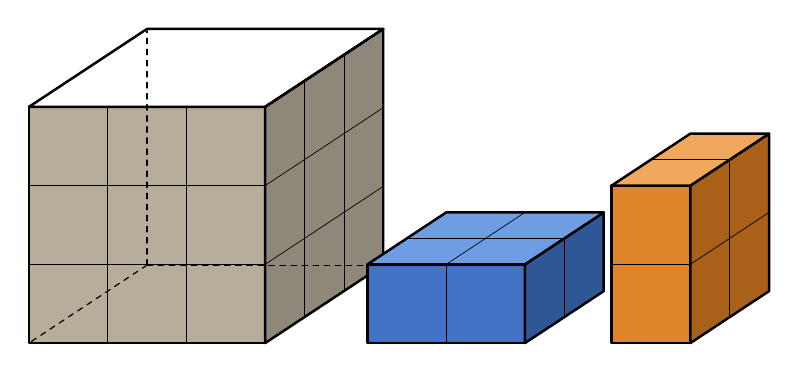
\begin{tikzpicture}[
  x={(1cm,0cm)}, y={(0.5cm,0.33cm)}, z={(0cm,1cm)},
  line join=round, line cap=round,
  edge/.style={line width=0.9pt},
  cell/.style={line width=0.25pt},
  hidden/.style={line width=0.45pt, dash pattern=on 2pt off 2pt},
]

% ── the empty 3×3×3 box: cardboard walls, open at the top ─────────────────
\begin{scope}
  \draw[edge, fill=cardfront] (0,0,0) -- (3,0,0) -- (3,0,3) -- (0,0,3) -- cycle;
  \draw[edge, fill=cardside]  (3,0,0) -- (3,3,0) -- (3,3,3) -- (3,0,3) -- cycle;

  \foreach \i in {1,2} {
    \draw[cell] (\i,0,0) -- (\i,0,3);   % front, vertical
    \draw[cell] (0,0,\i) -- (3,0,\i);   % front, horizontal
    \draw[cell] (3,\i,0) -- (3,\i,3);   % right, vertical
    \draw[cell] (3,0,\i) -- (3,3,\i);   % right, horizontal
  }

  % The mouth of the box — the rim only, no top face and no grid on it.
  \draw[edge] (0,0,3) -- (3,0,3) -- (3,3,3) -- (0,3,3) -- cycle;

  % Drawn last, over the cardboard: the three edges at the corner behind it.
  \draw[hidden] (0,3,0) -- (0,0,0);
  \draw[hidden] (0,3,0) -- (3,3,0);
  \draw[hidden] (0,3,0) -- (0,3,3);
\end{scope}

% ── a tile lying flat: 2 × 2 × 1. Solid — nothing shows through it ────────
\begin{scope}[shift={(4.3,0,0)}]
  \draw[edge, fill=bluefront] (0,0,0) -- (2,0,0) -- (2,0,1) -- (0,0,1) -- cycle;
  \draw[edge, fill=blueside]  (2,0,0) -- (2,2,0) -- (2,2,1) -- (2,0,1) -- cycle;
  \draw[edge, fill=bluetop]   (0,0,1) -- (2,0,1) -- (2,2,1) -- (0,2,1) -- cycle;

  \draw[cell] (1,0,0) -- (1,0,1);       % front
  \draw[cell] (2,1,0) -- (2,1,1);       % right
  \draw[cell] (1,0,1) -- (1,2,1);       % top, along y
  \draw[cell] (0,1,1) -- (2,1,1);       % top, along x
\end{scope}

% ── the same tile stood on its edge: 1 × 2 × 2 ────────────────────────────
\begin{scope}[shift={(7.4,0,0)}]
  \draw[edge, fill=orangefront] (0,0,0) -- (1,0,0) -- (1,0,2) -- (0,0,2) -- cycle;
  \draw[edge, fill=orangeside]  (1,0,0) -- (1,2,0) -- (1,2,2) -- (1,0,2) -- cycle;
  \draw[edge, fill=orangetop]   (0,0,2) -- (1,0,2) -- (1,2,2) -- (0,2,2) -- cycle;

  \draw[cell] (0,0,1) -- (1,0,1);       % front
  \draw[cell] (1,1,0) -- (1,1,2);       % right, vertical
  \draw[cell] (1,0,1) -- (1,2,1);       % right, horizontal
  \draw[cell] (0,1,2) -- (1,1,2);       % top
\end{scope}

\end{tikzpicture}
\end{document}
